% bp-ex-vo-vo.tex

\documentclass{standalone}
% newcommands.tex

\newcommand{\enq}{\texttt{enq}}
\newcommand{\deq}{\texttt{deq}}
\newcommand{\pput}{\texttt{PUT}}
\newcommand{\get}{\texttt{GET}}
\newcommand{\vs}{\texttt{vis}}
\newcommand{\so}{\texttt{so}}
\newcommand{\arb}{\texttt{ar}}
\newcommand{\rf}{\texttt{rf}}

% example
\newcommand{\po}[2]{\draw [->, thick] (#1) to node[above] {\Large{\so}} (#2);}
\newcommand{\pva}[2]{\draw [->, thick] (#1) to node[above] {$\Large{\so},\Large{\vs},\Large{\arb}$} (#2);}
\newcommand{\pbva}[2]{\draw [->, thick] (#1) to node[above] {$\Large{\so}$} node[below] {$\Large{\vs},\Large{\arb}$} (#2);}
\newcommand{\pv}[2]{\draw [->, thick] (#1) to node[above] {\Large{\so}} node[below] {\Large{\vs}} (#2);}
\newcommand{\evis}[2]{\draw [->, thick] (#1) to node[above, sloped, near end] {\Large{\vs}} (#2);}
\newcommand{\mvis}[2]{\draw [->, thick] (#1) to node[above, sloped] {\Large{\vs}} (#2);}
\newcommand{\ar}[2]{\draw [->, thick, allow upside down] (#1) to node[above, sloped] {\Large{\arb}} (#2);}
\newcommand{\va}[2]{\draw [->, thick, allow upside down] (#1) to node[above, sloped] {$\Large{\vs},\Large{\arb}$} (#2);}
\newcommand{\vab}[2]{\draw [->, thick, allow upside down] (#1) to node[below, sloped, near end] {$\Large{\vs},\Large{\arb}$} (#2);}
\newcommand{\vae}[2]{\draw [->, thick, allow upside down] (#1) to node[above, sloped, near end] {$\Large{\vs},\Large{\arb}$} (#2);}
\newcommand{\vas}[2]{\draw [->, thick, allow upside down] (#1) to node[sloped, near start, above] {$\Large{\vs},\Large{\arb}$} (#2);}

% serialization
\newcommand{\scc}[2]{\draw [->, very thick] (#1) to (#2);}
\newcommand{\rva}[2]{\draw [->, thick, allow upside down] (#1) to node[above, sloped] {$\Large{\rf},\Large{\vs},\Large{\arb}$} (#2);}
\newcommand{\rvb}[2]{\draw [->, thick, allow upside down] (#1) to node[below, sloped] {$\Large{\rf},\Large{\vs},\Large{\arb}$} (#2);}


\usepackage{tikz}
\usetikzlibrary{shapes, positioning, arrows.meta, decorations.pathmorphing}

\begin{document}
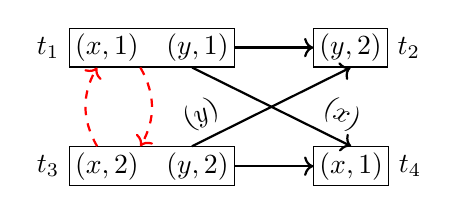
\begin{tikzpicture}[
  so/.style = {->, thick},
  wr/.style = {->, thick},
  co/.style = {->, thick},
  vo/.style = {->, thick},
  txn/.style = {draw, inner sep = 2pt}]

  % t1: W(x, 1) W(y, 1)
  \node[txn, label = left : $t_1$]
    (t1) {$\writeevent(x, 1) \quad \writeevent(y, 1)$};
  % t2: R(y, 2)
  \node[txn, right = 1.00cm of t1, label = right : $t_2$]
    (t2) {$\readevent(y, 2)$};
  % t3: W(x, 2) W(y, 2)
  \node[txn, below = 1.00cm of t1, label = left : $t_3$]
    (t3) {$\writeevent(x, 2) \quad \writeevent(y, 2)$};
  % t4: R(x, 1)
  \node[txn, right = 1.00cm of t3, label = right : $t_4$]
    (t4) {$\readevent(x, 1)$};

  % t1-SO-t2
  \draw[so] (t1) to node[above]{$\SO$} (t2);
  % t3-SO-t4
  \draw[so] (t3) to node[above]{$\SO$} (t4);
  % t1-WR-t4
  \draw[wr] (t1) to node[sloped, above, very near end]{$\WR(x)$} (t4.north);
  % t3-WR-t2
  \draw[wr] (t3) to node[sloped, above, very near start]{$\WR(y)$} (t2.south);

  % t1-VO-t3
  \draw[vo, dashed, red, bend left] (t1.-120) to node[]{$\VO$} (t3.120);
  % t3-VO-t1
  \draw[vo, dashed, red, bend left] (t3.160) to node[]{$\VO$} (t1.-160);
\end{tikzpicture}
\end{document}